\documentclass{article}

% import packages
\usepackage{amsmath,amsfonts,amsthm,amssymb,amsopn,bm}
\usepackage{mathtools}
\usepackage[margin=.9in]{geometry}
\usepackage{graphicx}
\usepackage[dvipsnames]{xcolor}
\usepackage{minted}
\usepackage{subcaption}
\usepackage{float}

% note command
\newcommand{\note}[1]{\textsf{\textcolor{Red}{#1}}}

% some math commands
\newcommand{\norm}[1]{\left\|#1\right\|}
\newcommand{\twonorm}[1]{\|#1\|_2^2}
\newcommand{\vect}[1]{\boldsymbol{#1}} % vector 
\DeclareMathOperator{\E}{\mathbb{E}}
\DeclareMathOperator{\R}{\mathbb{R}}
\DeclareMathOperator{\N}{\mathcal{N}}
\DeclareMathOperator{\cov}{Cov}
\DeclareMathOperator{\var}{Var}
\DeclareMathOperator{\grad}{\nabla\!}

% remove indents
\setlength\parindent{0px}
% enumerate with lowercase letters
\renewcommand{\theenumi}{\alph{enumi}}
% indented environment for solutions
\usepackage{changepage}
\newenvironment{solution}{\begin{adjustwidth}{8mm}{}}{\end{adjustwidth}}


% Homework title and date
\renewcommand{\title}{Homework 2}
\renewcommand{\date}{November 9, 2020}

\begin{document}

\begin{center}
        \LARGE \title \\ \vspace{10pt}
        \normalsize 
        Fall 2020, CSE 546: Machine Learning \\ \vspace{2pt}
        John Franklin Crenshaw \\ \vspace{2pt}
        \date
\end{center}

Collaborators: Robert Pecoraro, Samantha Tetef

\section*{Conceptual Questions}

\textbf{A0}
\begin{enumerate}
        \item This is not necessarily true.
        For example, if we have another highly correlated variable, like number of bathtubs, it could pick up the slack and provide the same info in principle.
        \item The constraining surface of the L1 norm has corners, unlike the L2 surface, which is a sphere.
        Generic loss functions will more likely ``hit'' this constraining surface at one of the corners, which corresponds to setting one or more weights equal to zero.
        As the L2 surface does not have corners, it does not generically favor sparsity.
        \item A potential upside: it more strongly encourages sparsity than the L1 norm, which may be desirable depending on the application.
        A potential downside: it is not a norm, nor is it convex, both of which are nice properties for a regularizer.
        \item True. A large step-size may cause the gradient-descent algorithm to diverge, or bounce back and forth around the minimum. 
        \item We do not need to calculate the gradient on the whole data set to decrease the loss.
        Instead we can estimate the gradient using a smaller subset of the data, which will give us a good idea of which ``direction'' to head in.
        Formally, it works because the expectation value of these stochastic gradients is the true gradient.
        \item One upside: SGD has smaller memory requirements, as you do not need to use the entire training set at once.
        One downside: the variance in gradients introduced by the random sampling can decrease the convergence rate.
\end{enumerate}


\section*{Convexity and Norms}

\textbf{A1}
\begin{enumerate}
        \item 
        Using the definition of the absolute value:
        \begin{align*}
                -|a| \leq a \leq |a| \\
                -|b| \leq b \leq |b|.
        \end{align*}
        Adding these, we have
        \begin{align*}
                -(|a| + |b|) \leq a + b \leq |a| + |b| \quad \Rightarrow \quad |a + b| \leq |a| + |b|,
        \end{align*}
        where again I applied the definition of the absolute value.
        Now, we have
        \begin{align*}
                f(x+y) =& \sum_i |x_i + y_i| \leq \sum_i |x_i| + |y_i| = f(x) + f(y) \\
                &\Rightarrow f(x+y) \leq f(x) + f(y).
        \end{align*}
        The other two properties are easier. 
        $f(x)$ is non-negative, as it is the sum of non-negative values, and the sum is only zero if every $x_i = 0$, i.e. $x = 0$.
        Finally,
        \begin{align*}
                f(ax) = \sum_i |a x_i| = |a| \sum_i |x_i| = |a| f(x).
        \end{align*}

        \item
        Let $n = 2$.
        We have
        \begin{align*}
                g(x) = \left( \sqrt{|x_1|} + \sqrt{|x_2|} \, \right)^2 = |x_1| + |x_2| + 2 \sqrt{|x_1||x_2|} \geq |x_1| + |x_2|.
        \end{align*}
        Thus the triangle inequality is broken whenever neither $x_1$ nor $x_2$ are zero.
\end{enumerate}

\textbf{B1}

Since $f : x \to x^2$ is a monotonically increasing map, we can establish these inequalities by comparing the squares of the values.
First, let us compare the one- and two-norms:
\begin{align*}
        \norm{x}_1^2 = \left( \sum_i |x_i| \right)^2 = \sum_i |x_i|^2 + \text{cross terms} \geq \sum_i |x_i|^2 = \left( \sqrt{\sum_i |x_i|^2} \right)^2 = \norm{x}_2^2,
\end{align*}
where I used the fact that all cross terms are products of non-negative numbers.
Now let us compare the two- and infinity-norms:
\begin{align*}
        \norm{x}_2^2 = \sum_i |x_i|^2 \geq ( \max_i |x_i| )^2 = \norm{x}_\infty,
\end{align*}
where I used the fact that all of the terms dropped from the sum are non-negative.
Putting these two inequalities together, we have
\begin{align*}
        \norm{x}_\infty \leq \norm{x}_2 \leq \norm{x}_1
\end{align*}


\textbf{A2}

I is not convex, as the line connecting b and c leaves the set.
II is convex, as the line connecting any two points is entirely contained within the set.
III is not convex, as the line connecting a and d leaves the set. \newline

\textbf{A3}

\begin{enumerate}
        \item This function is convex on this domain, as the line connecting any two points in this range lies above the function.
        \item This function is not convex on this domain, as the lines a $\to$ b and b $\to$ c lie below the function.
        \item This function is not convex on this domain, as the lines a $\to$ b, b $\to$ c, and a $\to$ c all lie below the function.
        \item This function is convex on this domain, as the line connecting any two paints in this range lies above the function.
\end{enumerate}

\textbf{B2}

\begin{enumerate}
        \item Applying the properties of a norm, we have
        \begin{align*}
                f(\lambda x + (1 - \lambda)y) = \norm{\lambda x + (1-\lambda)y} \leq \norm{\lambda x} + \norm{(1-\lambda)y} = \lambda \norm{x} + (1-\lambda)\norm{y} = \lambda f(x) + (1-\lambda)f(y),
        \end{align*}
        thus, all norms are convex.

        \item Using the result above,
        \begin{align*}
                \norm{\lambda x + (1-\lambda)y} \leq \lambda \norm{x} + (1-\lambda)\norm{y} \leq \lambda + (1-\lambda) = 1,
        \end{align*}
        where I used that $\norm{x}, \norm{y} \leq 1$.
        Therefore, the line connecting any two points is within radius one, and so is entirely in the set.
        Thus the set is convex.

        \item The set is not convex.
        For example, the line connecting any two adjacent `spikes' leaves the set.
        \begin{figure}[H]
                \begin{subfigure}{0.5\linewidth}
                        \centering
                        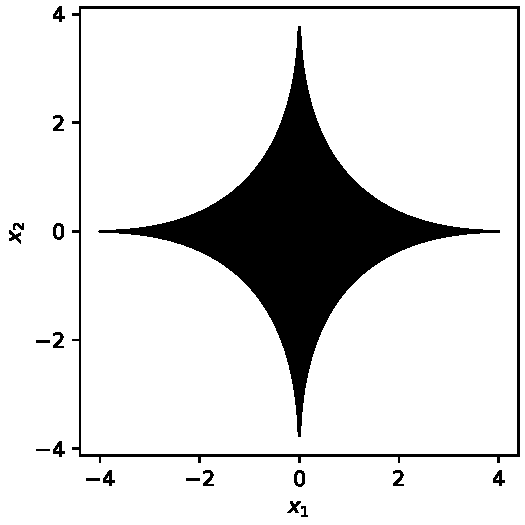
\includegraphics[width=\linewidth]{code/B2c.pdf}
                \end{subfigure}
                \hfill
                \begin{subfigure}{0.40\linewidth}
                        \centering
                        \begin{minted}[autogobble]{python}
                                fig, ax = plt.subplots(figsize=(3.5,3.5), 
                                                constrained_layout=True)
                                x = np.linspace(-4,4,1000)
                                y = (2 - np.sqrt(np.abs(x)))**2
                                ax.fill_between(x, -y, y, color='k')
                                ax.set(xlabel='$x_1$', ylabel='$x_2$',
                                yticks=[-4,-2,0,2,4])
                        \end{minted}
                \end{subfigure}
        \end{figure}
\end{enumerate}

\textbf{B3}

\begin{enumerate}
        \item
        Define $F(x) = \sum_i a_i f_i(x)$, where $a_i \in \R_{>0}$ and $\{f_i\}$ is a set of convex functions.
        Letting $\lambda \in [0,1]$, we have
        \begin{align*}
                F(\lambda x + (1-\lambda)y) 
                = \sum_i a_i f_i(\lambda x + (1-\lambda)y) \leq \sum_i \lambda \, a_i f_i(x) + (1-\lambda) \, a_i f_i(y) = \lambda F(x) + (1-\lambda) F(y),
        \end{align*}
        so $F$ is also convex.
        In other words, a positive-coefficient linear combination of convex functions is also a convex function.
        As the functions $\ell_i$ are convex, norms are convex, and $\lambda > 0$, it immediately follows that the given sum is convex.
        
        \item We prefer convex loss functions, because they are easy to minimize, as any local minima we find are guaranteed to be global minima.
        
\end{enumerate}

\newpage

\section*{Lasso on a real dataset}

\textbf{A4}

\begin{enumerate}
        \item \, \newline \vspace{-1.5cm}
        \begin{center}
                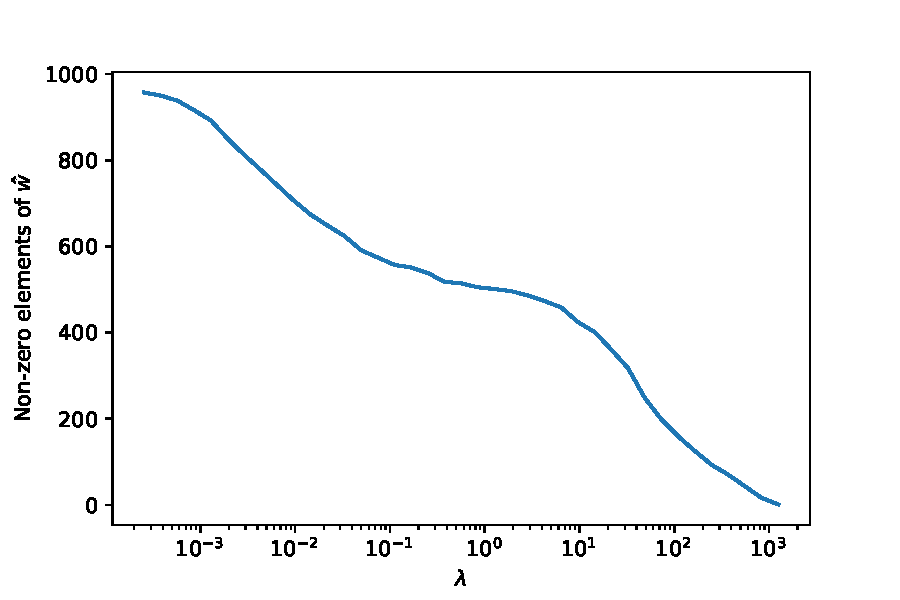
\includegraphics[width=0.7\textwidth]{code/A4a.pdf}
        \end{center}

        \item \, \newline \vspace{-1.5cm}
        \begin{center}
                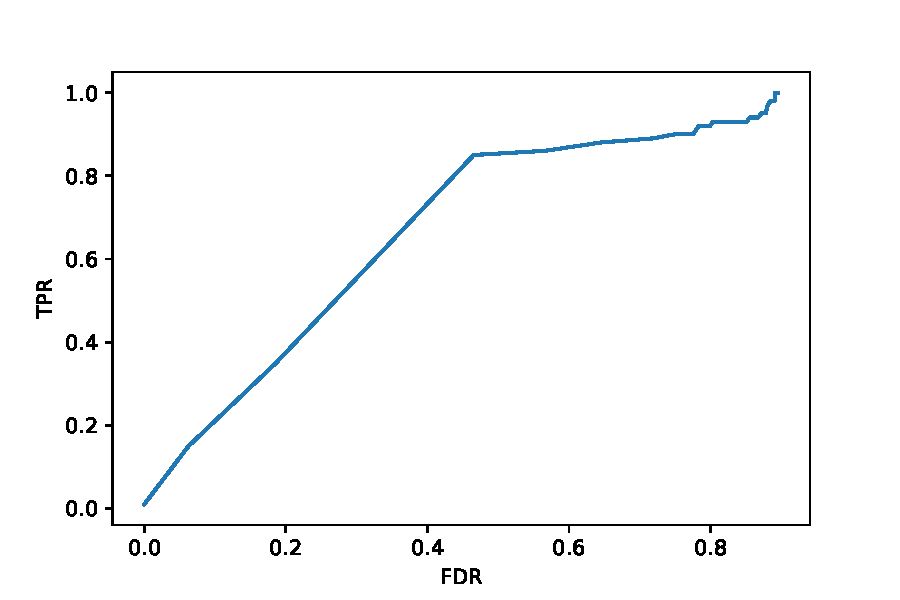
\includegraphics[width=0.7\textwidth]{code/A4b.pdf}
        \end{center}

        \item We start with $\lambda$ at a value that forces all elements of $\hat{w}$ to zero.
        As we decrease $\lambda$, we decrease the regularization (i.e. we decrease the amount by which $\hat{w}$ s driven towards zero), which results in more and more non-zero elements in $\hat{w}$.
        In part a, we can see that this relationship is approximately a power law.
        In part b, decreasing $\lambda$ corresponds to following the curve from bottom left to top right.
        High $\lambda$ means few false detections, but also a low true positive rate.
        As you decrease $\lambda$, you make more positive detections, but unfortunately the false detection rate increases as well.
        Luckily, the TPR outpaces the FDR until TPR is around 0.8.
        After this point, further decreasing $\lambda$ quickly increases the FDR with little improvement to the TPR.

        Below is the Lasso code used to generate these plots
        \begin{minted}[autogobble]{python}
                # set params
                n = 500
                d = 1000
                k = 100
                sig = 1
                
                # generate data
                np.random.seed(0)
                X = np.random.normal(0, 1, (n,d))
                w = np.arange(1,d+1)/k; w[k:] = 0
                y = np.random.normal(X @ w, sig)
                
                # initialize model
                wH = np.zeros(len(w)) # w hat
                bH = 0 # b hat
                
                # set initial values
                lam = max(np.abs(2 * X.T @ (y - y.mean()))) # initial lambda
                sparsity = 0 # set initial sparsity
                
                # values to save
                lambdas = []
                sparsities = []
                fdr = []
                tpr = []
                
                # pre-calculate values
                a = 2*(X**2).sum(axis=0)
                
                # regularization path
                while sparsity <= 0.95*d:
                    
                    dwH = np.ones(len(w)) # set initial dwH
                    
                    # coordinate descent
                    while max(dwH) > 1e-5:
                        
                        # save old wH
                        wH_old = wH.copy()
                
                        # update bH
                        bH = np.mean(y - X @ wH)
                        
                        for i in range(d):
                            
                            wH_ = wH.copy(); wH_[i] = 0
                            c = 2 * (X[:,i] * (y - (bH + X @ wH_))).sum()
                            
                            c = c if np.abs(c) > lam else 0
                            wH[i] = (c - np.sign(c)*lam)/a[i]
                            
                        dwH = np.abs(wH - wH_old)
                        
                    # save values
                    lambdas.append(lam)
                    sparsity = len(wH[np.abs(wH) > 0])
                    sparsities.append(sparsity)
                    fdr.append( len(wH[(w == 0) & (wH != 0)]) / np.clip(len(wH[wH!= 0]), 1, None) )
                    tpr.append( len(wH[(w != 0) & (wH != 0)]) / k )
                    
                    # new lambda
                    lam /= 1.5 
                        \end{minted}
\end{enumerate}

\newpage

\textbf{A5}

Pre-questions
\begin{enumerate}
        \item (i) The percent of people using public transportation is dependent on many policy decisions, such as the cost of public transit and the expansiveness of the public transit system.
        (ii) The number of homeless people counted in the street is dependent on the number and quality of homeless shelters in the city, as well as the many policy choices that impact the economic realities of living in the city.
        (iii) The number and kinds of drugs seized depends on policy choices such as which drugs are considered illegal (e.g. in 2020, whether or not marijuana is illegal depends on which state you live in).

        \item (i) The number of households with only one parent might be interpreted as a reason for high crime, but could also be the result of violent crime if those crimes result in the deaths of parents.
        (ii) Low incomes could be construed as the cause of crime, but it is also possible that people with low-incomes are forced to live in areas with more crime as the property values there are lower.
        (iii) The number of vacant houses could be a cause of crime (e.g. providing locations in which violent crimes can be committed), but could also be the result, if people are leaving the community due to the high crime rate.
\end{enumerate}

Lasso Model
\begin{enumerate}
        \item \, \newline \vspace{-1.5cm}
        \begin{center}
                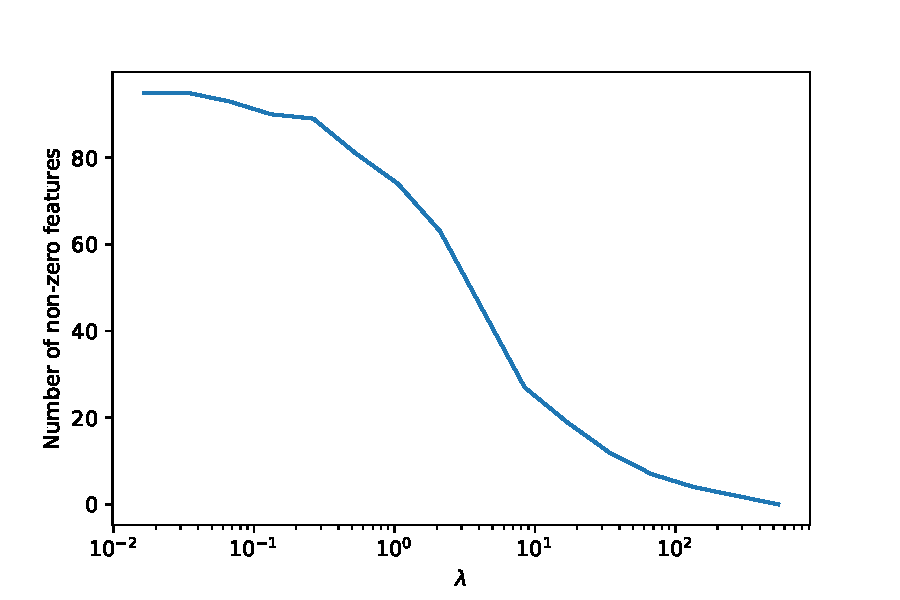
\includegraphics[width=0.7\textwidth]{code/A5a.pdf}
        \end{center}

        \item \, \newline \vspace{-1.5cm}
        \begin{center}
                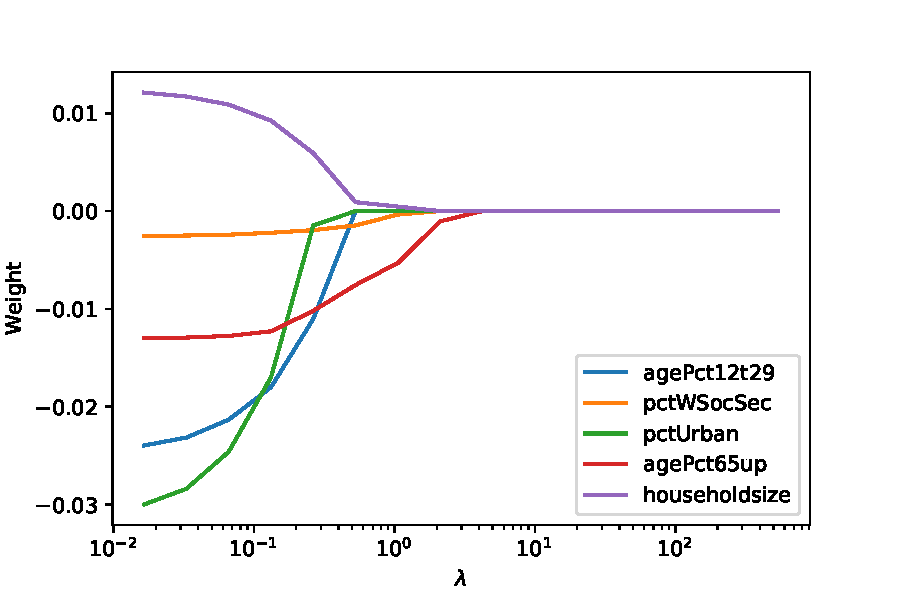
\includegraphics[width=0.7\textwidth]{code/A5b.pdf}
        \end{center}

        \item \, \newline \vspace{-1.5cm}
        \begin{center}
                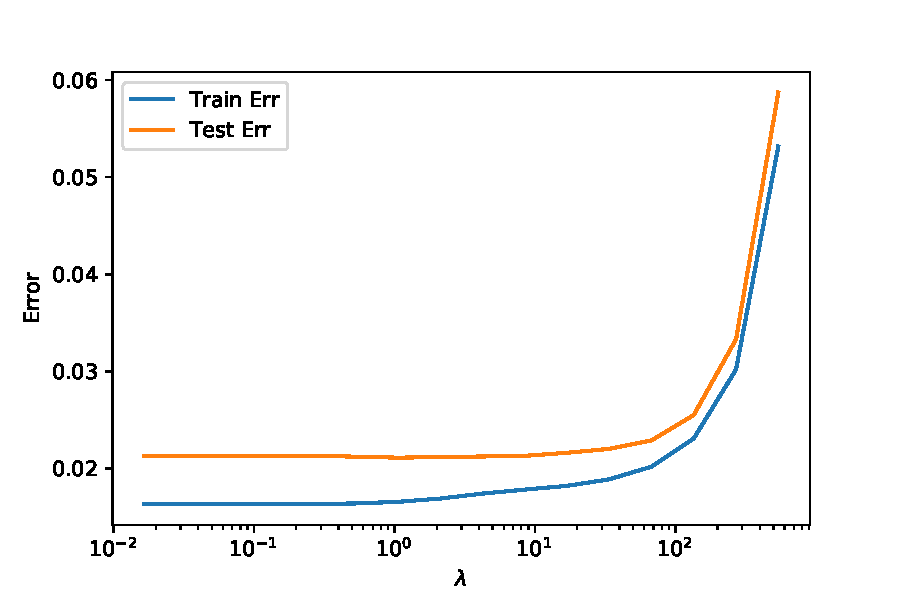
\includegraphics[width=0.7\textwidth]{code/A5c.pdf}
        \end{center}

        \item The feature with the greatest positive weighting is \texttt{NumIlleg}, the number of children born to never-married parents, and the greatest negative weighting is \texttt{PctFam2Par}, the percentage of families headed by two parents.
        These two weights appear to be telling the same story -- communities where children are raised by two parents tend to have less violent crime.
        However, as the pre-questions indicate, one must be careful when attempting to draw conclusions about causality from these weights.
        It might be that single-parent households and high violent crime rates are both the result of a deeper underlying cause.

        \item This policy makes the assumption of a causal relationship -- i.e. that the presence of people over 65 leads to lower crime.
        However, a simple Lasso regression cannot tell us about causation, only correlation.
        To illustrate this point, imagine a world in which no one over the age of 65 commits violent crime.
        Then a retirement community will likely have no crime, as almost everyone in the community is over the age of 65.
        However, the lack of crime is not due to the presence of the older people, but rather the absence of younger people.
        In this scenario, introducing older people to a high-crime community does not negate the presence of young crime-committing people in the community, and so would not help reduce crime.

        \, \newline
        Here is the Lasso code used to calculate the values plotted above:
        \begin{minted}{python}
X = df_train.drop('ViolentCrimesPerPop', axis = 1).values
y = df_train['ViolentCrimesPerPop'].values

Xtest = df_test.drop('ViolentCrimesPerPop', axis = 1).values
ytest = df_test['ViolentCrimesPerPop'].values

d = X.shape[1]

# initialize model
wH = np.zeros(d) # w hat
bH = 0 # b hat

# set initial values
lam = max(np.abs(2 * X.T @ (y - y.mean()))) # initial lambda
sparsity = 0 # set initial sparsity

# values to save
lambdas = []
sparsities = []
variables = ['agePct12t29',
             'pctWSocSec',
             'pctUrban',
             'agePct65up',
             'householdsize']
regpaths = {var:[] for var in variables}
trainerr = []
testerr = []

# pre-calculate values
a = 2*(X**2).sum(axis=0)

# regularization path
while lam >= 0.01:
    
    dwH = np.ones(len(w)) # set initial dwH
    
    # coordinate descent
    while max(dwH) > 1e-5:
        
        # save old wH
        wH_old = wH.copy()

        # update bH
        bH = np.mean(y - X @ wH)
        
        for i in range(d):
            
            wH_ = wH.copy(); wH_[i] = 0
            c = 2 * (X[:,i] * (y - (bH + X @ wH_))).sum()
            
            c = c if np.abs(c) > lam else 0
            wH[i] = (c - np.sign(c)*lam)/a[i]
            
        dwH = np.abs(wH - wH_old)
        
    # save values
    lambdas.append(lam)
    sparsity = len(wH[np.abs(wH) > 0])
    sparsities.append(sparsity)
    for var in variables:
        idx = df_train.columns.get_loc(var)
        regpaths[var].append(wH[idx])
    trainerr.append(((y - bH - X @ wH)**2).mean())
    testerr.append(((ytest - bH - Xtest @ wH)**2).mean())
    
    print(f'{sparsity:<4}{lam:>7.2f}')
    
    # new lambda
    lam /= 2
        \end{minted}
\end{enumerate}

\newpage

\section*{Logistic Regression}

\textbf{A6}

\begin{enumerate}
        \item First the $w$ gradient:
        \begin{align*}
                \grad_w J(w,b) &= \frac{1}{n} \sum_{i=1}^n -y_i x_i^T \frac{\exp(-y_i(b + x_i^Tw))}{1 + \exp(-y_i(b + x_i^Tw))} + 2 \lambda w \\
                &= \frac{1}{n} \sum_{i=1}^n -y_i x_i^T \left( 1 - \frac{1}{1 + \exp(-y_i(b + x_i^Tw))} \right) + 2 \lambda w \\
                &= \frac{1}{n} \sum_{i=1}^n \, y_i x_i^T \, ( \, \mu_i(w,b) - 1 \, ) + 2 \lambda w           
        \end{align*}
        Now the $b$ gradient will be almost identical, except we lose the factor of $x_i^T$ in the first term, and the second term goes to zero.
        Thus, we have
        \begin{align*}
                \grad_b J(w,b) = \frac{1}{n} \sum_{i=1}^n \, y_i \, ( \, \mu_i(w,b) - 1 \, )
        \end{align*}

        \item Here are the plots:
        \begin{center}
                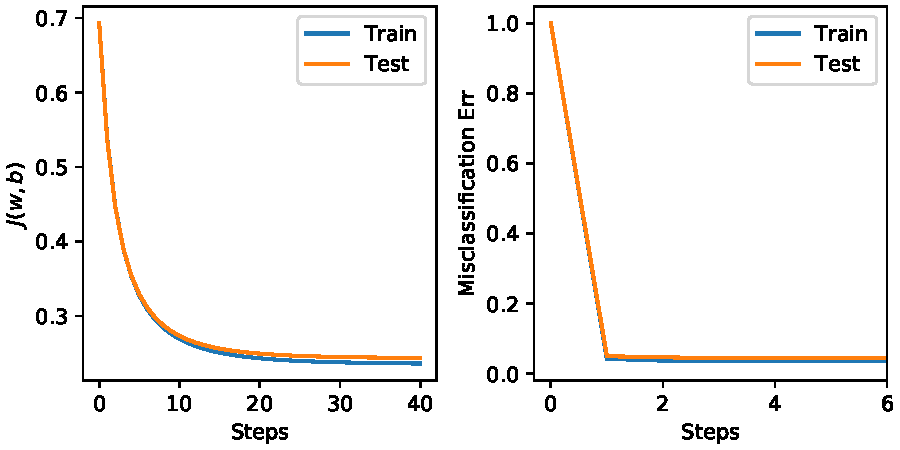
\includegraphics[width=0.7\textwidth]{code/A6b.pdf}
        \end{center}
        Interestingly, while the loss $J(w,b)$ is still decreasing for tens of steps, using the simple classification rule, we essentially reach maximum accuracy with only a single step (using step size 0.1).

        \item Here are the plots using a batch size of 1.
        \begin{center}
                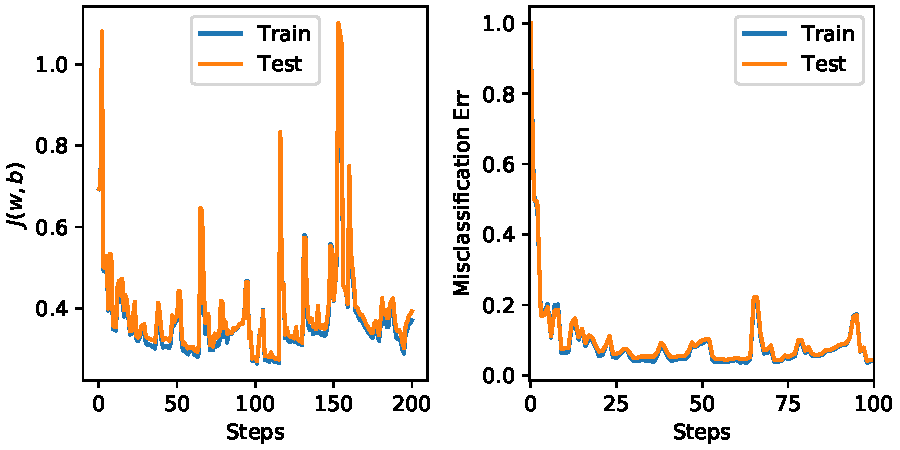
\includegraphics[width=0.7\textwidth]{code/A6c.pdf}
        \end{center}
        You can see that the estimator still trains and can reasonably well classify digits, but the loss function is relatively unstable.
        In addition, the performance doesn't monotonically increase: there are gradient steps that decrease the accuracy.
        Performing gradient descent on one image at a time is not super effective, as the gradient with respect to one image is not a good estimate of the total gradient.

        \item Here are the plots using a batch size of 100.
        \begin{center}
                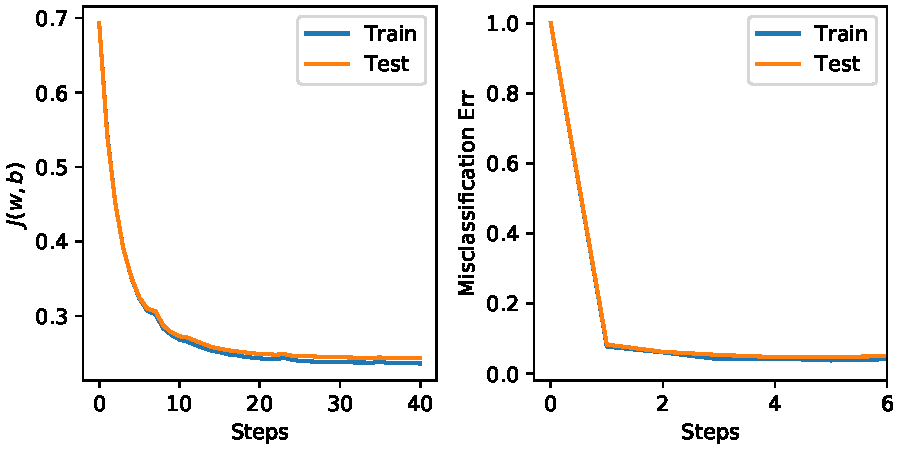
\includegraphics[width=0.7\textwidth]{code/A6d.pdf}
        \end{center}
        This looks very similar to the regular gradient descent, just with a few small bumps in the loss function.
        Clearly, a batch size of 100 provides a far better estimate of the total gradient than only the gradient with respect to a single image.
\end{enumerate}

\newpage

\textbf{B4}

\begin{enumerate}
        \item 
        \begin{align*}
                \frac{\partial \mathcal{L}}{\partial w^{(m)}} 
                &= - \sum_{i=1}^n \sum_{\ell=1}^k \mathbf{1}\{y_i=\ell\} \left( x_i \delta_{\ell,m} - \frac{x_i \exp(w^{(m)}x_i)}{\sum_{j=1}^k \exp(w^{(j)} x_i)} \right) \\
                &= - \sum_{i=1}^n x_i \left( y_{i,m} - \texttt{softmax}(w^{(m)}x_i) \right),
        \end{align*}
        where in the second line, I used that $\sum_\ell \mathbf{1}\{y_i=\ell\}\delta_{\ell,m}$ is the $m$th element of the one-hot encoding of $y_i$.
        Now that we have the $m$th element of $\grad_W \mathcal{L}(W)$, we can use the definition of $\hat{y}$ to immediately write down the vectorized solution:
        \begin{align*}
                \grad_W \mathcal{L}(W) = - \sum_{i=1}^n x_i (y_i - \hat{y}_i^{(W)})^T.
        \end{align*}

        \item This one is easier, as we can apply the same matrix calculus rules we used when we studied ordinary least squares.
        In particular, using $\grad_v \norm{v}_2^2 = \grad_v v^T v = 2 v$ and $\grad_W W^T x = x$, we have
        \begin{align*}
                \grad_W J(W) = - \sum_{i=1}^n x_i (y_i - W^T x_i)^T,
        \end{align*}
        where we can deduce the placement of the transpose via the fact that $\grad_W J(W)$ is a matrix.

        \item Here is a table of classification accuracies for the training and test set, for the solutions trained with the two loss functions, $\mathcal{L}(W)$ and $J(W)$:
        \begin{center}
                \begin{tabular}{l c c}
                        \, & \multicolumn{2}{c}{Accuracy} \\
                        Loss Function & Training & Test\vspace{1mm}\\
                        $\mathcal{L}(W)$ & 0.903 & 0.908 \\ 
                        $J(W)$ & 0.851 & 0.856 \\
               \end{tabular}
        \end{center}
        We can see that the loss function $\mathcal{L}(W)$ is better for this problem.
        Here are the training curves for the two solutions as well, showing that the two solutions have approximately converged:
        \begin{figure}[h]
                \centering
                \begin{subfigure}{0.45\textwidth}
                        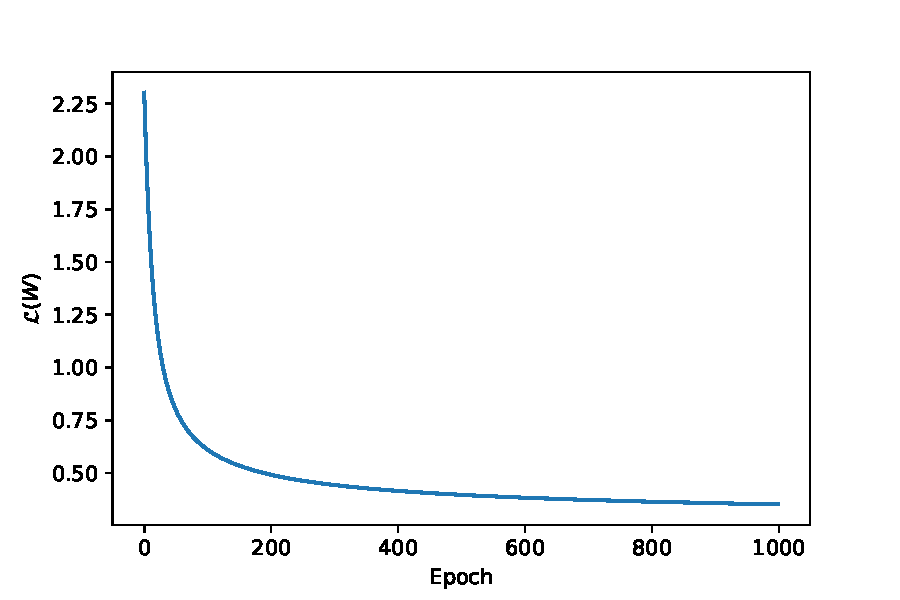
\includegraphics[width=\textwidth]{code/B4_celoss.pdf}
                \end{subfigure}
                \begin{subfigure}{0.45\textwidth}
                        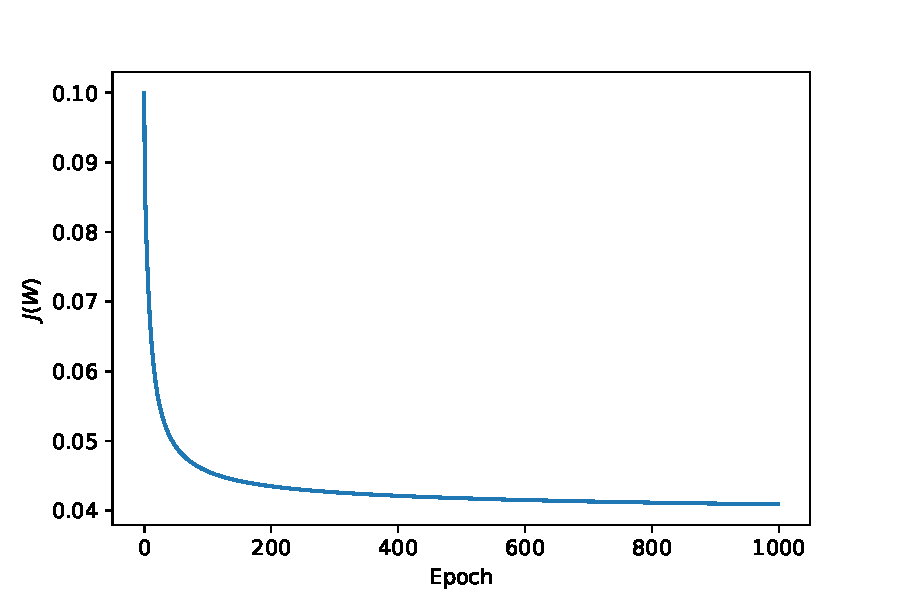
\includegraphics[width=\textwidth]{code/B4_mseloss.pdf}
                \end{subfigure}
        \end{figure}

        These solutions are the result of the following code:
        \begin{minted}{python}
import torch
from mnist import MNIST

def load_dataset():
    mndata = MNIST('../../../python-mnist/data/')
    X_train, labels_train = map(np.array, mndata.load_training())
    X_test, labels_test = map(np.array, mndata.load_testing())
    X_train = X_train/255.0
    X_test = X_test/255.0
    
    return X_train, labels_train, X_test, labels_test

X_train, Y_train, X_test, Y_test = load_dataset()

X_train = torch.Tensor(X_train)
y_train = torch.Tensor(Y_train).long()
X_test = torch.Tensor(X_test)
y_test = torch.Tensor(Y_test).long()

epochs = 1000
step_size = 0.1
W = torch.zeros(784, 10, requires_grad=True)
ce_loss = []
for epoch in range(epochs):
    y_hat = torch.matmul(X_train, W)
    # cross entropy combines softmax calculation with NLLLoss
    loss = torch.nn.functional.cross_entropy(y_hat, y_train)
    ce_loss.append(loss)
    # computes derivatives of the loss with respect to W
    loss.backward()
    # gradient descent update
    W.data = W.data - step_size * W.grad
    # .backward() accumulates gradients into W.grad instead
    # of overwriting, so we need to zero out the weights
    W.grad.zero_()

y_hat = torch.matmul(X_train, W).argmax(axis=1)
softmax_acc_train = len(y_train[(y_hat == y_train)])/len(y_train)

y_hat = torch.matmul(X_test, W).argmax(axis=1)
softmax_acc_test = len(y_test[(y_hat == y_test)])/len(y_test)


W = torch.zeros(784, 10, requires_grad=True)
mse_loss = []
step_size = 0.1
epochs = 1000
for epoch in range(epochs):
    y_hat = torch.matmul(X_train, W)
    # this time use MSE loss
    loss = torch.nn.functional.mse_loss(y_hat, torch.nn.functional.one_hot(y_train).float())
    mse_loss.append(loss)
    # computes derivatives of the loss with respect to W
    loss.backward()
    # gradient descent update
    W.data = W.data - step_size * W.grad
    # .backward() accumulates gradients into W.grad instead
    # of overwriting, so we need to zero out the weights
    W.grad.zero_()

y_hat = torch.matmul(X_train, W).argmax(axis=1)
mse_acc_train = len(y_train[(y_hat == y_train)])/len(y_train)

y_hat = torch.matmul(X_test, W).argmax(axis=1)
mse_acc_test = len(y_test[(y_hat == y_test)])/len(y_test)
        \end{minted}
\end{enumerate}


\section*{Confidence Interval of Least Squares Estimation}

\textbf{B5}

\begin{enumerate}
        \item We are given inputs $X$ and observations $Y \sim \N(X\beta^*, I)$.
        %We can estimate $\beta^*$ with the least-squares estimator $\hat{\beta} = (X^T X)^{-1} X^T Y$.
        From the notes, we know that if $Y \sim \N(\mu, \Sigma)$ then $AY + b \sim \N(A\mu + b, A \Sigma A^T)$.
        Setting $A = (X^T X)^{-1} X^T$ and $b=0$, and using the least-squares estimator $\hat{\beta} = (X^T X)^{-1} X^T Y$, we have
        \begin{align*}
                \hat{\beta} &\sim \N((X^T X)^{-1} X^T X \beta^*, (X^T X)^{-1} X^T X (X^T X)^{-1}) \sim \N(\beta^*, (X^T X)^{-1})
        \end{align*}
        
        \item 
        If we let $\beta^* = 0$, then we have $\hat{\beta}_j \sim \N(0,(X^T X)_{jj}^{-1})$.
        From the notes, we know that 
        \begin{align*}
                P(\hat{\beta}_j \geq t) \leq \exp \left( -\frac{t^2}{2(X^T X)_{jj}^{-1}} \right).
        \end{align*}
        If we set this probability bound equal to $\delta$, we have
        \begin{align*}
                t = \sqrt{2 (X^T X)_{jj}^{-1} \log(1/\delta)}.
        \end{align*}
        Therefore,
        \begin{align*}
                P \left( \hat{\beta}_j \geq \sqrt{2 (X^T X)_{jj}^{-1} \log(1/\delta)} \, \right) \leq \delta.
        \end{align*}
        From symmetry, we have
        \begin{align*}
                P \left( |\hat{\beta}_j| \geq \sqrt{2 (X^T X)_{jj}^{-1} \log(1/\delta)} \, \right) \leq 2\delta.
        \end{align*}
        Making the substitution $\delta \to \delta/2$, we have
        \begin{align*}
                P \left( |\hat{\beta}_j| \geq \sqrt{2 (X^T X)_{jj}^{-1} \log(2/\delta)} \, \right) \leq \delta.
        \end{align*}
        or equivalently
        \begin{align*}
                P \left( |\hat{\beta}_j| \leq \sqrt{2 (X^T X)_{jj}^{-1} \log(2/\delta)} \, \right) \geq 1 - \delta.
        \end{align*}
        We cannot put this bound on all elements of $\hat{\beta}$ simultaneously because the derivation comes from the integral of a one-dimensional Gaussian.
        If we want to put bounds on all the elements of $\hat{\beta}$, we need to sum over all dimensions and redefine $\delta \to \delta/d$ (see part d).

        \item As $x_i = \sqrt{(i \!\!\mod d) + 1} ~ e_{(i \!\!\mod d) + 1}$, we have
        \begin{align*}
                (X^T X)_{jk} 
                = \sum_i^{n} X_{ij} X_{ik} 
                = \sum_i^{n} [(i \!\!\!\!\mod d) + 1] \delta_{j,(i \!\!\!\!\mod d) + 1} \delta_{k,(i \!\!\!\!\mod d) + 1}
        \end{align*}
        \vspace{-5mm}
        \begin{align*}
                \Longrightarrow (X^T X)_{jj} 
                = (j + 1) \sum_i^{n} \delta_{j,(i \!\!\!\!\mod d) + 1}.
        \end{align*}
        Let's assume (as in our case) that $n$ is divisible by $d$, then the sum evaluates to $n/d$, so we have 
        \begin{align*}
                (X^T X)_{jj} = (1 + j) \frac{n}{d} \Longrightarrow (X^T X)_{jj}^{-1} = \frac{d}{n (1+j)}.
        \end{align*}
        Now we can plot the elements of $\hat{\beta}$:
        \begin{center}
                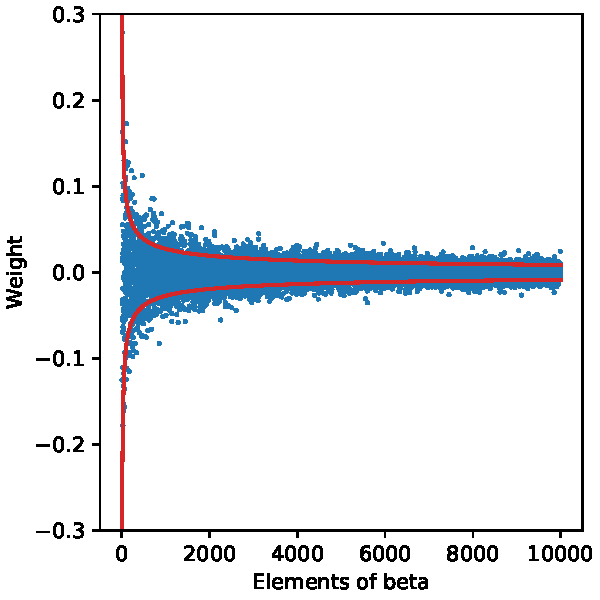
\includegraphics[width=0.5\textwidth]{code/B5d.pdf}
        \end{center}
        22\% of the weights are outside the confidence interval.

        The code for this problem follows:
        \begin{minted}{python}
n = 20000
d = 10000

X = []
for i in range(0,n):
    j = i % d
    x = np.zeros(d)
    x[j] = np.sqrt(j + 2)
    X.append(x)
X = np.array(X)

np.random.seed(0)
Y = np.random.normal(0, 1, n)

XTY = X.T @ Y

beta = d/(n*(1 + np.arange(1,d+1))) * XTY
gamma = np.sqrt(2 * d/(n*(1 + np.arange(1,d+1))) * np.log(2/0.95))

nabove = len(beta[np.abs(beta) > gamma])
print(nabove/d)
        \end{minted}






        \item Using the union bound, have
        \begin{align*}
                P(\cup_i E_i) \leq \sum_{i=1}^m P(E_i) \leq \sum_{i=1}^m \delta = m \delta.
        \end{align*}
        Thus, if we pick new bounds $\gamma_i$ for each $P(E_i)$ such that $P(E_i) \leq \delta / m$, then $P(\cup_i E_i) \leq \delta$.
        This is equivalent to redefining $\delta \to \delta/d$ in the equations of part b.
        Thus, we have the bound
        \begin{align*}
                \gamma_j = \sqrt{2(X^T X)_{j,j}^{-1} \log(2d/\delta)}.
        \end{align*}
\end{enumerate}



\end{document}
